\documentclass[12pt,a4paper]{article}

%\usepackage[left=1.5cm,right=1.5cm,top=1cm,bottom=2cm]{geometry}
\usepackage[in, plain]{fullpage}
\usepackage{array}
\usepackage{../../../pas-math}
\usepackage{../../../moncours}


%\usepackage{pas-cours}
%-------------------------------------------------------------------------------
%          -Packages nécessaires pour écrire en Français et en UTF8-
%-------------------------------------------------------------------------------
\usepackage[utf8]{inputenc}
\usepackage[frenchb]{babel}
\usepackage[T1]{fontenc}
\usepackage{lmodern}
\usepackage{textcomp}



%-------------------------------------------------------------------------------

%-------------------------------------------------------------------------------
%                          -Outils de mise en forme-
%-------------------------------------------------------------------------------
\usepackage{hyperref}
\hypersetup{pdfstartview=XYZ}
%\usepackage{enumerate}
\usepackage{graphicx}
\usepackage{multicol}
\usepackage{tabularx}
\usepackage{multirow}


\usepackage{anysize} %%pour pouvoir mettre les marges qu'on veut
%\marginsize{2.5cm}{2.5cm}{2.5cm}{2.5cm}

\usepackage{indentfirst} %%pour que les premier paragraphes soient aussi indentés
\usepackage{verbatim}
\usepackage{enumitem}
\usepackage[usenames,dvipsnames,svgnames,table]{xcolor}

\usepackage{variations}

%-------------------------------------------------------------------------------


%-------------------------------------------------------------------------------
%                  -Nécessaires pour écrire des mathématiques-
%-------------------------------------------------------------------------------
\usepackage{amsfonts}
\usepackage{amssymb}
\usepackage{amsmath}
\usepackage{amsthm}
\usepackage{tikz}
\usepackage{xlop}
%-------------------------------------------------------------------------------



%-------------------------------------------------------------------------------


%-------------------------------------------------------------------------------
%                    - Mise en forme avancée
%-------------------------------------------------------------------------------

\usepackage{ifthen}
\usepackage{ifmtarg}


\newcommand{\ifTrue}[2]{\ifthenelse{\equal{#1}{true}}{#2}{$\qquad \qquad$}}

%-------------------------------------------------------------------------------

%-------------------------------------------------------------------------------
%                     -Mise en forme d'exercices-
%-------------------------------------------------------------------------------
%\newtheoremstyle{exostyle}
%{\topsep}% espace avant
%{\topsep}% espace apres
%{}% Police utilisee par le style de thm
%{}% Indentation (vide = aucune, \parindent = indentation paragraphe)
%{\bfseries}% Police du titre de thm
%{.}% Signe de ponctuation apres le titre du thm
%{ }% Espace apres le titre du thm (\newline = linebreak)
%{\thmname{#1}\thmnumber{ #2}\thmnote{. \normalfont{\textit{#3}}}}% composants du titre du thm : \thmname = nom du thm, \thmnumber = numéro du thm, \thmnote = sous-titre du thm

%\theoremstyle{exostyle}
%\newtheorem{exercice}{Exercice}
%
%\newenvironment{questions}{
%\begin{enumerate}[\hspace{12pt}\bfseries\itshape a.]}{\end{enumerate}
%} %mettre un 1 à la place du a si on veut des numéros au lieu de lettres pour les questions 
%-------------------------------------------------------------------------------

%-------------------------------------------------------------------------------
%                    - Mise en forme de tableaux -
%-------------------------------------------------------------------------------

\renewcommand{\arraystretch}{1.7}

\setlength{\tabcolsep}{1.2cm}

%-------------------------------------------------------------------------------



%-------------------------------------------------------------------------------
%                    - Racourcis d'écriture -
%-------------------------------------------------------------------------------

% Angles orientés (couples de vecteurs)
\newcommand{\aopp}[2]{(\vec{#1}, \vec{#2})} %Les deuc vecteurs sont positifs
\newcommand{\aopn}[2]{(\vec{#1}, -\vec{#2})} %Le second vecteur est négatif
\newcommand{\aonp}[2]{(-\vec{#1}, \vec{#2})} %Le premier vecteur est négatif
\newcommand{\aonn}[2]{(-\vec{#1}, -\vec{#2})} %Les deux vecteurs sont négatifs

%Ensembles mathématiques
\newcommand{\naturels}{\mathbb{N}} %Nombres naturels
\newcommand{\relatifs}{\mathbb{Z}} %Nombres relatifs
\newcommand{\rationnels}{\mathbb{Q}} %Nombres rationnels
\newcommand{\reels}{\mathbb{R}} %Nombres réels
\newcommand{\complexes}{\mathbb{C}} %Nombres complexes


%Intégration des parenthèses aux cosinus
\newcommand{\cosP}[1]{\cos\left(#1\right)}
\newcommand{\sinP}[1]{\sin\left(#1\right)}


%Probas stats
\newcommand{\stat}{statistique}
\newcommand{\stats}{statistiques}
%-------------------------------------------------------------------------------

%-------------------------------------------------------------------------------
%                    - Mise en page -
%-------------------------------------------------------------------------------

\newcommand{\twoCol}[1]{\begin{multicols}{2}#1\end{multicols}}


\setenumerate[1]{font=\bfseries,label=\textit{\alph*})}
\setenumerate[2]{font=\bfseries,label=\arabic*)}


%-------------------------------------------------------------------------------
%                    - Elements cours -
%-------------------------------------------------------------------------------





%\makeatletter
%\renewcommand*{\@seccntformat}[1]{\csname the#1\endcsname\hspace{0.1cm}}
%\makeatother


%\author{Olivier FINOT}
\date{}
\title{Proportionnalité}

%\newcommand{\disp}{false}

%\lhead{CH1 : Stats et représentations graphiques}
%\rhead{O. FINOT}
%
%\rfoot{Page \thepage}
\begin{document}
%\maketitle

\chap[num=1, color=red]{Proportionnalité}{Olivier FINOT, \today }

\section{Situation de proportionnalité}

\begin{mydefs}
	\begin{itemize}
		\item 	Deux grandeurs sont \kw{en situation de proportionnalité} lorsque les suites de nombres qui correspondent à leurs mesures sont \kw{proportionnelles}.
		
		\item Dans un tableau, si les valeurs d'une lignes s'obtiennent en \kw{multipliant} ou en \kw{divisant} celles de l'autre ligne par un \kw{même nombre} (noté \kw{$k$}); alors les suites de nombres présentées dans ce tableau sont proportionnelles. $k$ est le \kw{coefficient de proportionnalité} .
		
		\item Lorsque les grandeurs proportionnelles sont présentées sous forme de \kw{graphique}, les points correspondant à ces deux grandeurs sont alignés sur une droite qui passe par l'origine du repère. 
		
	\end{itemize}

	
\end{mydefs}

\begin{myraps}
	\begin{itemize}
		\item Dans un repère \kw{orthogonal} le plan est défini par deux axes perpendiculaires.
		\item L'axe horizontal est l'\kw{axe des abscisses}.
		\item L'axe vertical est l'\kw{axe des ordonnées}.
		\item Les \kw{coordonnées} d'un point du plan sont constituées d'un couple de nombres \kw{$(x;y)$} où $x$ est une valeur sur l'axe des abscisses et $y$ sur l'axe des ordonnées.
		\item Leur point d'intersection est l'\kw{origine} du repère.
	\end{itemize}
\end{myraps}

\begin{myexs}
	\begin{enumerate}
		\item 	Soit ($u_n$) la suite arithmétique de terme initial $u_0 = 1,5$ et de raison $r = -7$.
		
		Le terme de rang $n$ est $u_n = 1,5 + n \times (-7)$ c'est à dire $u_n=1,5 - 7n$.
		
		On a ainsi : 
		\begin{itemize}
			\item $u_4 = 1,5 - 7 \times 4 = -26,5$
			\item $u_{100} = 1,5 - 7 \times 100 = -698,5$
		\end{itemize}
		
		\item Soit ($u_n$) la suite arithmétique de terme initial $u_1 = 14$ et de raison $r = 1,3$.
		
		Le terme de rang $n$ est $u_n = 14 + (n-1) \times 1,3$; c'est à dire $u_n = 12,7 + 1,3n$.

		On a ainsi : 
		\begin{itemize}
			\item $u_4 = 12,7 + 1,3 \times 4 = 17,9$;
			\item $u_{100} = 12,7 + 1,3 \times 100 = 142,7$.
		\end{itemize}
	\end{enumerate}

	
	
\end{myexs}

\section{Recherche d'un quatrième proportionnelle}

\begin{mymeth}{}
	L'égalité $\dfrac{a}{b}=\dfrac{c}{d}$ est une proportion.\\
	
	La règle du \kw{produit en croix} permet de calculer un des quatre nombres ($a$, $b$, $c$ ou $d$) si les trois autres sont connus :
	
	\begin{center}
		Si $\dfrac{a}{b} = \dfrac{c}{d}$ alors $a \times d = b \times c$
	\end{center}
\end{mymeth}

\begin{myex}
	La droite d'ajustement obtenue grâce au tableur passe par le point moyen $G$ dont nous avons calculé les coordonnées.
	\begin{center}
		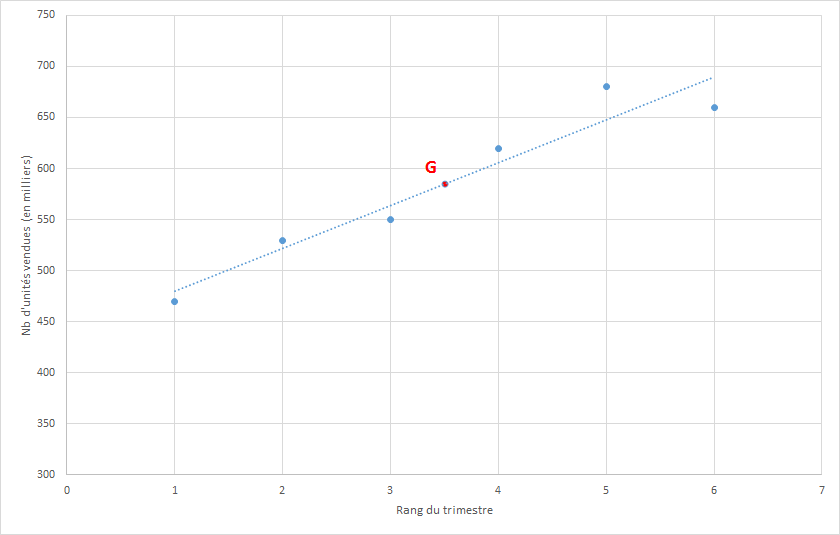
\includegraphics[scale =0.7]{./img/graph2}		
	\end{center}

\end{myex}


\section{Pourcentages}

\subsection{Taux de pourcentage}
\begin{mydef}
	%	\begin{itemize}
	%		\item 
	Un \kw{taux de pourcentage} $t\, \% $ correspond à une fraction du type $\dfrac{t}{100}$ où $t$ est un nombre quelconque. Il peut également s'écrire sous la forme du nombre décimal obtenu en divisant $t$ par $100$.
	
	%	\end{itemize}
\end{mydef}

\subsection{Calculer un taux de pourcentage}
\begin{mymeth}
	Pour calculer le \kw{taux de pourcentage} que représente en e grandeur $B$ par rapport à une grandeur $A$, on applique la formule :
	
	\begin{center}
		\kw{$Taux_{grandeurB/grandeurA} = \dfrac{grandeur B \times 100}{grandeur A}$}
	\end{center}
	
\end{mymeth}

\begin{myex}
	Pendant les soldes, un article valant 110 € bénéficie une réduction de 44 €.
	
	Calcul du \kw{taux de réduction} : $\dfrac{44 \times 100}{110} = 40$\\
	
	L'article bénéficie d'une réduction de $40\,\%$
\end{myex}

\subsection{Prendre un pourcentage d'une quantité}
\begin{mymeth}
	Pour calculer \kw{$t\, \%$} d'une quantité, on \kw{multiplie} cette quantité par \kw{$\dfrac{t}{100}$}.
	
\end{mymeth}

\begin{myex}
	Pendant les soldes, un autre article, valant 55 € bénéficie d'une réduction de 15 $\%$.
	
	Calcul de 15 $\%$ de 55 : $55 \times \dfrac{15}{100} = 55 \times 0,15 = 8,25$.\\
	
	Le \kw{montant} de la réduction est 8,25 €.
\end{myex}	
\end{document}